\documentclass[aspectratio=169,9pt]{beamer}

\usetheme{default}
\usecolortheme{default}
\usefonttheme{professionalfonts}
\setbeamertemplate{navigation symbols}{}
\setbeamertemplate{footline}{%
  \hfill\usebeamerfont{footline}\insertframenumber\,/\,\inserttotalframenumber\hspace{1em}\vspace{0.5em}
}
\setbeamercolor{block title}{bg=blue!10!white, fg=blue!60!black}
\setbeamercolor{block body}{bg=blue!4!white}
\setbeamercolor{alerted text}{fg=red!70!black}

\usepackage{amsmath,amssymb,amsthm}
\usepackage{mathtools}
\usepackage{tikz}
\usetikzlibrary{positioning,arrows.meta,calc}
\usepackage{booktabs}
\usepackage{xcolor}
\usepackage{colortbl}
\usepackage{graphicx}
\usepackage{siunitx}

%% ── Semantic colours ────────────────────────────────────────────────────────
\definecolor{trueblue}{RGB}{21,101,192}
\definecolor{falsered}{RGB}{198,40,40}
\definecolor{ignorgray}{RGB}{97,97,97}
\definecolor{contramber}{RGB}{230,81,0}
\definecolor{midpurple}{RGB}{57,73,171}
\definecolor{lightgray}{RGB}{240,240,240}

%% ── Macros ──────────────────────────────────────────────────────────────────
\newcommand{\tv}[2]{\langle #1,#2 \rangle}
\newcommand{\tvt}[1]{\langle #1 \rangle}
\newcommand{\VM}{V_{\mathcal{M}}}
\newcommand{\semp}{[\![p]\!]}
\newcommand{\BBL}{{B_{\mathrm{BL}}}}
\newcommand{\boxop}{[\![\Box p]\!]}
\newcommand{\diaop}{[\![\Diamond p]\!]}
\newcommand{\D}{\mathcal{D}}
\newcommand{\TRUE}{\textcolor{trueblue}{\textsc{True}}}
\newcommand{\FALSE}{\textcolor{falsered}{\textsc{False}}}
\newcommand{\IGN}{\textcolor{ignorgray}{\textsc{Ign}}}
\newcommand{\CONT}{\textcolor{contramber}{\textsc{Cont}}}

%% ── Title ───────────────────────────────────────────────────────────────────
\title{$\mathbf{B}_{\mathbf{BL}}$: A Bilateral Modal Logic\\[4pt]for LLM Factuality Evaluation}
\author{Bradley Allen}
\institute{University of Amsterdam}
\date{TLLM 2026}

\begin{document}

\begin{frame}
  \titlepage
\end{frame}

%% ════════════════════════════════════════════════════════════════════════════
%% SLIDE 1 — Introduction: The Wrong Question
%% ════════════════════════════════════════════════════════════════════════════
\begin{frame}{The Wrong Question}

  \begin{block}{Prevailing approach to LLMs and logic}
    \textit{Can we get LLMs to reason logically?}\\[2pt]
    \small Make the model do modus ponens, avoid contradictions, chain inferences.
  \end{block}

  \bigskip\pause

  \begin{alertblock}{Our approach}
    \textit{Can we build a logic that reasons \textbf{using} LLMs?}
  \end{alertblock}

  \bigskip\pause

  \begin{block}{LLMs as defeasible derivability oracles}
    Sources that provide \textbf{provisional}, \textbf{non-monotone} verdicts about what
    is epistemically supportable — embedded in a logical calculus that makes those
    verdicts \textbf{compositionally tractable}.
  \end{block}

  \bigskip\pause
  \small
  The locus of inference is the \emph{framework}, not the model.
  The LLM answers bilateral verification queries; the logic does everything else.

\end{frame}

%% ════════════════════════════════════════════════════════════════════════════
%% SLIDE 1b — What BBL Accomplishes
%% ════════════════════════════════════════════════════════════════════════════
\begin{frame}{Two Contributions}

  \begin{block}{Contribution 1: $V_3 \times V_3$ is the right semantic space}
    Current LLM factuality evaluation treats verification as a single dimension~---
    true, false, or uncertain ($V_3$).
    But \textbf{verifiability} and \textbf{refutability} are empirically independent.
    Collapsing them loses information: ignorance $\tv{f}{f}$ and contradiction
    $\tv{t}{t}$ are both ``uncertain'' in $V_3$ but have completely different
    epistemic profiles.  $V_3{\times}V_3$ preserves the distinction.
  \end{block}

  \bigskip

  \begin{block}{Contribution 2: $\Box p$ operationalises prompt-agnostic knowledge}
    Correct evaluation at a single phrasing~$s_0$ may not reflect genuine knowledge.
    $[\![\Box p]\!] = \langle\min u_i,\max v_i\rangle$ formalises
    \textbf{reliable knowledge}: the bilateral truth value must be stable across
    semantic variations of the question.
    Prompt-sensitive knowledge~(PSK) --- $\semp \in D$ but $[\![\Box p]\!]\notin D$
    --- is the formal safety-relevant gap.
  \end{block}

\end{frame}

%% ════════════════════════════════════════════════════════════════════════════
%% SLIDE 2 — Object Language
%% ════════════════════════════════════════════════════════════════════════════
\begin{frame}{$\BBL$: Object Language}

  \textbf{Syntax.}\quad Propositional atoms $p,q,\ldots$ closed under:
  \[
    \varphi \;::=\; p \;\mid\; \neg\varphi \;\mid\; \varphi\wedge\psi
                \;\mid\; \varphi\vee\psi \;\mid\; \Box\varphi \;\mid\; \Diamond\varphi
  \]

  \medskip\pause

  \textbf{Truth-value components.}\quad
  $V_3 = \{f,\, e,\, t\}$ with $f <_t e <_t t$
  \hfill
  (\textit{false / indeterminate / true})

  \medskip\pause

  \textbf{Bilateral truth value.}\quad
  $\tv{u}{v} \in V_3 \times V_3$ where:
  \begin{itemize}
    \item $u$ = \textbf{verifiability}: degree to which $p$ is supportable
    \item $v$ = \textbf{refutability}: degree to which $\neg p$ is supportable
  \end{itemize}

  \medskip\pause

  \textbf{LLM-grounded valuation.}\quad
  $\semp = \tv{u}{v}$ via two \emph{independent} queries:
  \[
    u \;=\; \zeta^+(s_0, p)
    \qquad\qquad
    v \;=\; \zeta^-(s_0, p)
  \]
  each by majority vote over $n=3$ samples.
  The components are independent by design — the oracle is queried twice.

\end{frame}

%% ════════════════════════════════════════════════════════════════════════════
%% SLIDE 2b — Truth Functions
%% ════════════════════════════════════════════════════════════════════════════
\begin{frame}{Truth Functions}

  \begin{columns}[T]
    \column{0.48\textwidth}
    \textbf{Propositional connectives}
    \begin{align*}
      \neg\tv{u}{v}
        &= \tv{v}{u} \\[6pt]
      \tv{u_1}{v_1} \wedge \tv{u_2}{v_2}
        &= \tv{\min(u_1,u_2)}{\max(v_1,v_2)} \\[4pt]
      \tv{u_1}{v_1} \vee \tv{u_2}{v_2}
        &= \tv{\max(u_1,u_2)}{\min(v_1,v_2)}
    \end{align*}

    \smallskip
    \textit{Negation} swaps components:\\
    refutability of $p$ = verifiability of $\neg p$.

    \column{0.48\textwidth}
    \textbf{Modal operators} over accessible situations $\{s_i\}$
    \begin{align*}
      [\![\Box p]\!]
        &= \tv{\displaystyle\min_i u_i}{\displaystyle\max_i v_i} \\[8pt]
      [\![\Diamond p]\!]
        &= \tv{\displaystyle\max_i u_i}{\displaystyle\min_i v_i}
    \end{align*}

    \smallskip
    \textit{Necessity} is conservative:\\
    weakest verification, strongest refutation across situations.
  \end{columns}

  \bigskip\pause

  \begin{block}{Compositional semantics for the oracle}
    Conjunction propagates weakness: if either conjunct carries refutation
    evidence, the compound inherits it.
    $[\![\Box p]\!]$ filters out prompt-sensitive verdicts before they
    enter any inference chain.
  \end{block}

\end{frame}

%% ════════════════════════════════════════════════════════════════════════════
%% SLIDE 3 — The Bilattice NINE
%% ════════════════════════════════════════════════════════════════════════════
\begin{frame}{The Bilattice \textsc{Nine}}

  $\textsc{Nine} = \langle V_3{\times}V_3,\;\leq_t,\;\leq_k\rangle$
  carries two independent lattice orderings:

  \[
    \tv{u_1}{v_1} \leq_t \tv{u_2}{v_2}
      \;\Leftrightarrow\; u_1 \leq u_2 \;\text{ and }\; v_1 \geq v_2
    \qquad\quad
    \tv{u_1}{v_1} \leq_k \tv{u_2}{v_2}
      \;\Leftrightarrow\; u_1 \leq u_2 \;\text{ and }\; v_1 \leq v_2
  \]

  \smallskip
  \hfill{\small $\leq_t$: \textbf{truth} ordering \quad $\leq_k$: \textbf{knowledge/information} ordering}

  \medskip

  \begin{columns}[c]
    \column{0.52\textwidth}
    \centering
    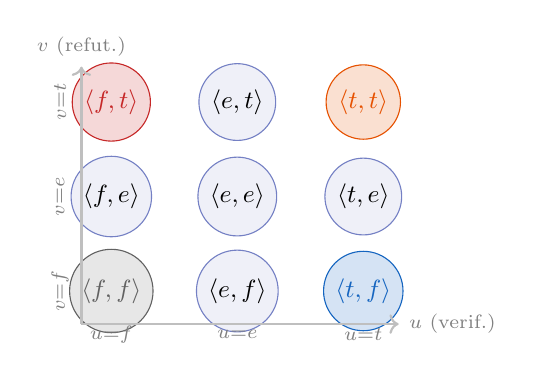
\begin{tikzpicture}[scale=1.0,
      base/.style={circle,draw,inner sep=2.5pt,font=\small},
      T/.style={base,draw=trueblue,fill=trueblue!18,text=trueblue,font=\small\bfseries},
      F/.style={base,draw=falsered,fill=falsered!18,text=falsered,font=\small\bfseries},
      I/.style={base,draw=ignorgray,fill=ignorgray!15,text=ignorgray,font=\small\bfseries},
      C/.style={base,draw=contramber,fill=contramber!18,text=contramber,font=\small\bfseries},
      M/.style={base,draw=midpurple!70,fill=midpurple!8,font=\small},
    ]
      % Grid: x=u (f,e,t), y=v (t→top, f→bottom)
      \node[F] (ft) at (0,2.4) {$\tv{f}{t}$};
      \node[M] (et) at (1.6,2.4) {$\tv{e}{t}$};
      \node[C] (tt) at (3.2,2.4) {$\tv{t}{t}$};

      \node[M] (fe) at (0,1.2) {$\tv{f}{e}$};
      \node[M] (ee) at (1.6,1.2) {$\tv{e}{e}$};
      \node[M] (te) at (3.2,1.2) {$\tv{t}{e}$};

      \node[I] (ff) at (0,0)   {$\tv{f}{f}$};
      \node[M] (ef) at (1.6,0) {$\tv{e}{f}$};
      \node[T] (tf) at (3.2,0) {$\tv{t}{f}$};

      % Axis labels
      \foreach \x/\lbl in {0/$u{=}f$, 1.6/$u{=}e$, 3.2/$u{=}t$}
        \node[font=\scriptsize,gray] at (\x,-0.55) {\lbl};
      \foreach \y/\lbl in {0/$v{=}f$, 1.2/$v{=}e$, 2.4/$v{=}t$}
        \node[font=\scriptsize,gray,rotate=90] at (-0.65,\y) {\lbl};
      \draw[->,gray!50,thick] (-0.38,-0.42) -- (3.65,-0.42)
        node[right,font=\scriptsize,gray]{$u$ (verif.)};
      \draw[->,gray!50,thick] (-0.38,-0.42) -- (-0.38,2.85)
        node[above,font=\scriptsize,gray]{$v$ (refut.)};
    \end{tikzpicture}

    \column{0.44\textwidth}
    \small
    \begin{tabular}{@{}ll@{}}
      \toprule
      Value & Semantics \\
      \midrule
      \textcolor{trueblue}{$\tv{t}{f}$}
        & \textbf{True}: verified, not refuted \\[3pt]
      \textcolor{falsered}{$\tv{f}{t}$}
        & \textbf{False}: refuted, not verified \\[3pt]
      \textcolor{ignorgray}{$\tv{f}{f}$}
        & \textbf{Ignorance}: no signal \\[3pt]
      \textcolor{contramber}{$\tv{t}{t}$}
        & \textbf{Contradiction}: conflicting \\[3pt]
      \multicolumn{2}{@{}l@{}}{\textcolor{midpurple}{$\tv{t}{e}$, $\tv{e}{f}$, \ldots}
        \quad partial / asymmetric} \\
      \bottomrule
    \end{tabular}

    \bigskip
    \small
    $\tv{f}{f}$ and $\tv{t}{t}$ are both
    ``uncertain'' under unilateral evaluation.
    \textbf{$\BBL$ makes the distinction} —
    and it is diagnostically consequential.
  \end{columns}

\end{frame}

%% ════════════════════════════════════════════════════════════════════════════
%% SLIDE 4 — The LLM-Grounded Model MM
%% ════════════════════════════════════════════════════════════════════════════
\begin{frame}{The LLM-Grounded Model $\mathcal{M}$}

  \[
    \mathcal{M} \;=\; \langle S,\; R_\mathcal{M},\; V_\mathcal{M} \rangle
  \]

  \begin{columns}[T]
    \column{0.48\textwidth}
    \begin{block}{$S$ — Situations}
      Natural-language descriptions: source questions, paraphrases, reorderings.
      $s_0 \in S$ is the \textbf{source situation} (the original question/claim context).
    \end{block}

    \medskip

    \begin{block}{$R_\mathcal{M}$ — Accessibility}
      Meaning-preserving syntactic variation:\\
      $s_0\, R_\mathcal{M}\, s_i$ iff $s_i$ is a paraphrase of $s_0$.\\[2pt]
      \small Generated once per dataset via Claude~Opus~4.6; cached and shared across all evaluation models.
    \end{block}

    \column{0.48\textwidth}
    \begin{block}{$V_\mathcal{M}$ — Bilateral Valuation}
      $V_\mathcal{M}(s, p) = \tv{u}{v}$ via two independent LLM queries:
      \begin{align*}
        u &= \zeta^+(s,p) \;\; \text{(verification)} \\
        v &= \zeta^-(s,p) \;\; \text{(refutation)}
      \end{align*}
      \small Each by majority vote over $n=3$ calls to:\\
      C$^+$: \textit{``Is $p$ supported by evidence?''}\\
      C$^-$: \textit{``Is $\neg p$ supported by evidence?''}
    \end{block}
  \end{columns}

  \bigskip
  \small
  The LLM is an oracle for $V_\mathcal{M}$. It is never asked to infer.
  All reasoning is done by the formal calculus over the $\tv{u}{v}$ values it returns.

\end{frame}

%% ════════════════════════════════════════════════════════════════════════════
%% SLIDE 5 — Epistemic Policies as D-Parameterisation
%% ════════════════════════════════════════════════════════════════════════════
\begin{frame}{Epistemic Policies as $\BBL_{D,D^*}$ Parameterisation}

  The \textbf{projection operator} maps $\tv{u}{v}$ to a classical verdict:
  \[
    \pi_{D,D^*}\!\bigl(\tv{u}{v}\bigr) \;=\;
    \begin{cases}
      \mathbf{true}   & \text{if } \tv{u}{v} \in D \quad\text{(designated)} \\
      \mathbf{false}  & \text{if } \tv{u}{v} \in D^* \quad\text{(anti-designated)} \\
      \mathbf{abstain}& \text{otherwise (gap)}
    \end{cases}
  \]

  \medskip

  \small
  \begin{center}
  \begin{tabular}{ll@{\quad}l@{\quad}l}
    \toprule
    \textbf{Policy} & $D$ & $D^*$ & \textbf{Character} \\
    \midrule
    Classical
      & $\{\tv{t}{f}\}$
      & $\{\tv{f}{t}\}$
      & Only clean verified assertions designated \\[3pt]
    Paraconsistent
      & $\{\tv{t}{f},\, \tv{t}{t}\}$
      & $\{\tv{f}{t},\, \tv{e}{t}\}$
      & Tolerates contradictions; designates all verified \\[3pt]
    Paracomplete
      & $\{\tv{t}{f},\, \tv{t}{e}\}$
      & $\{\tv{f}{t}\}$
      & Tolerates gaps; designates partial verifications \\
    \bottomrule
  \end{tabular}
  \end{center}

  \medskip\pause

  \begin{block}{Key insight}
    \small Classical, paraconsistent, and paracomplete evaluation are not ad hoc thresholds
    — they are instances of $\BBL_{D,D^*}$, differing \emph{only} in the
    choice of designated values.
    The policy is a \textbf{logical parameter}, not an engineering choice.
  \end{block}

\end{frame}

%% ════════════════════════════════════════════════════════════════════════════
%% SLIDE 6 — Knowledge Stability and the Modal Operator
%% ════════════════════════════════════════════════════════════════════════════
\begin{frame}{Knowledge Stability: The Modal Operator $\Box$}

  \textbf{Modal necessity} aggregates $\semp$ over $s_0$ and $n$ paraphrase
  situations $\{s_1,\ldots,s_n\}$:
  \[
    [\![\Box p]\!] \;=\;
    \Bigl\langle\,
      \min_t\{u_i\},\;
      \max_t\{v_i\}
    \,\Bigr\rangle
    \qquad
    i = 0, 1, \ldots, n
  \]

  \begin{columns}[T]
    \column{0.52\textwidth}
    \textbf{Epistemological reading:}\\[4pt]
    $[\![\Box p]\!] \in D$ iff $p$ is verifiable and not refuted across
    \emph{all} syntactically accessible situations.

    \medskip
    This implements the \textbf{safety condition} (Sosa/Williamson) and
    \textbf{tracking condition} (Nozick) from epistemology:
    knowledge requires that the verdict would not easily have been different
    in nearby situations.

    \column{0.44\textwidth}
    \textbf{Operationally:}
    \begin{enumerate}\setlength\itemsep{3pt}
      \item Generate $n$ paraphrases of $s_0$
      \item Evaluate $\semp$ at each $s_i$
      \item Aggregate: take $\min$ verifiability, $\max$ refutability
    \end{enumerate}

    \medskip\small
    Necessity is \emph{conservative}: any single situation
    that refutes $p$ pulls $[\![\Box p]\!]$ away from $\tv{t}{f}$.
  \end{columns}

  \medskip\pause

  \begin{block}{Modal possibility $\Diamond$}
    \small $[\![\Diamond p]\!] = \langle\max_t\{u_i\},\, \min_t\{v_i\}\rangle$ — $p$ is supportable
    from \emph{at least one} accessible situation.
    The B~axiom $p \to \Box\Diamond p$ connects the two: stable truth implies
    witnessed possibility.
  \end{block}

\end{frame}

%% ════════════════════════════════════════════════════════════════════════════
%% SLIDE 7 — Prompt-Sensitive Knowledge
%% ════════════════════════════════════════════════════════════════════════════
\begin{frame}{Prompt-Sensitive Knowledge (PSK)}

  \begin{alertblock}{Definition}
    $p$ is \textbf{prompt-sensitive knowledge} at $s_0$ if\\[4pt]
    \hspace{2em}$\semp \in D$ \quad but \quad $[\![\Box p]\!] \notin D$
  \end{alertblock}

  \medskip

  The model \emph{appears} to know $p$ at $s_0$ but the verdict does not survive
  syntactic variation.

  \bigskip

  \textbf{Why PSK is not genuine knowledge:}
  \small
  \begin{itemize}\setlength\itemsep{3pt}
    \item \textbf{Fails safety} (Sosa/Williamson): the model would have produced
          a different verdict in a nearby accessible situation
    \item \textbf{Fails tracking} (Nozick): the mechanism is sensitive to
          surface form, not semantic content
    \item \textbf{Fails reliabilism}: the process is not truth-conducive across
          the relevant reference class of inputs
  \end{itemize}

  \medskip\pause

  \begin{columns}[T]
    \column{0.48\textwidth}
    \begin{block}{PSK is diagnostic}
      PSK signals \emph{where} the model's knowledge is fragile — a target for
      fine-tuning, retrieval augmentation, or explicit uncertainty.
    \end{block}
    \column{0.48\textwidth}
    \begin{block}{$[\![\Box p]\!]$ is the filter}
      Inference chains should be built on $[\![\Box p]\!] \in D$, not
      $\semp \in D$.
      Modal stability is the right epistemic threshold for reasoning.
    \end{block}
  \end{columns}

\end{frame}

%% ════════════════════════════════════════════════════════════════════════════
%% SLIDE — How C+ and C- Are Computed
%% ════════════════════════════════════════════════════════════════════════════
\begin{frame}[fragile]{How $\zeta^+$ and $\zeta^-$ Are Computed}

  \begin{columns}[T]

    \column{0.48\textwidth}
    \textbf{Verification query} $\zeta^+$ (forced-choice):
    \smallskip

    \setbeamercolor{block body}{bg=trueblue!6}
    \begin{block}{}
      \ttfamily\footnotesize
      You are tasked with determining whether
      the following assertion can be verified as
      true based on available evidence and
      knowledge.

      \smallskip
      Assertion: \textit{The answer to ``In
      Severance, whom does Mark Scout replace
      as department head?'' is Peter ``Petey''
      Kilmer.}

      \smallskip
      Context: \textit{In Severance, whom does
      Mark Scout replace as department head?}

      \smallskip
      You must respond with exactly one of:
      \textbf{VERIFIED}
      \textbf{CANNOT VERIFY}

      \smallskip
      Response:
    \end{block}
    \smallskip
    \footnotesize
    \begin{tabular}{ll}
      \textbf{VERIFIED} & $\to\; u = t$ \\
      \textbf{CANNOT VERIFY} & $\to\; u = f$ \\
      \textit{parse failure} & $\to\; u = e$
    \end{tabular}

    \column{0.48\textwidth}
    \textbf{Refutation query} $\zeta^-$ (forced-choice):
    \smallskip

    \setbeamercolor{block body}{bg=falsered!6}
    \begin{block}{}
      \ttfamily\footnotesize
      You are tasked with determining whether
      the following assertion can be refuted
      (shown to be false) based on available
      evidence and knowledge.

      \smallskip
      Assertion: \textit{The answer to ``In
      Severance, whom does Mark Scout replace
      as department head?'' is Peter ``Petey''
      Kilmer.}

      \smallskip
      Context: \textit{In Severance, whom does
      Mark Scout replace as department head?}

      \smallskip
      You must respond with exactly one of:
      \textbf{REFUTED}
      \textbf{CANNOT REFUTE}

      \smallskip
      Response:
    \end{block}
    \smallskip
    \footnotesize
    \begin{tabular}{ll}
      \textbf{REFUTED} & $\to\; v = t$ \\
      \textbf{CANNOT REFUTE} & $\to\; v = f$ \\
      \textit{parse failure} & $\to\; v = e$
    \end{tabular}

  \end{columns}

  \smallskip
  \footnotesize
  Issued $n=3$ times each; majority vote $\Rightarrow \semp=\tv{u}{v}$.
  Parse failure ($e$) = model could not commit.
  Components are \textbf{entirely independent}: the model never sees both questions.

\end{frame}

%% ════════════════════════════════════════════════════════════════════════════
%% SLIDE EX-A — Example: Stable True
%% ════════════════════════════════════════════════════════════════════════════
\begin{frame}{Example: Stable Knowledge \hfill \small Qwen~2.5~72B $\times$ SimpleQA}

  \begin{block}{Assertion (ground truth: \textcolor{trueblue}{correct})}
    \textit{The answer to ``Who was the lawyer who developed matrix algebra and
    also worked on higher-dimensional geometry?'' is \textbf{Arthur Cayley}.}
  \end{block}

  \medskip

  \begin{columns}[T]
    \column{0.52\textwidth}
    \footnotesize
    \begin{tabular}{l p{3.4cm} l}
      \toprule
      Sit. & Paraphrase & $\semp$ \\
      \midrule
      $s_0$ & \textit{Who was the lawyer who developed matrix algebra\ldots?}
              & \textcolor{trueblue}{$\tv{t}{f}$} \\[3pt]
      $s_1$ & \textit{Which lawyer is known to have developed matrix algebra\ldots?}
              & \textcolor{trueblue}{$\tv{t}{f}$} \\[3pt]
      $s_2$ & \textit{Who was the attorney who developed matrix algebra\ldots?}
              & \textcolor{trueblue}{$\tv{t}{f}$} \\[3pt]
      $s_3$ & \textit{Can you identify the lawyer responsible for matrix algebra\ldots?}
              & \textcolor{trueblue}{$\tv{t}{f}$} \\
      \bottomrule
    \end{tabular}

    \column{0.44\textwidth}
    \begin{align*}
      [\![\Box p]\!]
        &= \langle\min(t,t,t,t),\\
        &\hspace{1.5em}\max(f,f,f,f)\rangle\\
        &= \textcolor{trueblue}{\tv{t}{f}}
    \end{align*}

    \smallskip
    $\semp \in D$ \;\textbf{and}\; $[\![\Box p]\!] \in D$

    \smallskip
    \begin{block}{}
      \small\textbf{Stable knowledge.}
      The verdict $\tv{t}{f}$ is robust across all four
      situations — not prompt-sensitive.
    \end{block}
  \end{columns}

\end{frame}

%% ════════════════════════════════════════════════════════════════════════════
%% SLIDE EX-B — Example: Prompt-Sensitive Knowledge (PSK)
%% ════════════════════════════════════════════════════════════════════════════
\begin{frame}{Example: Prompt-Sensitive Knowledge \hfill \small Qwen~2.5~72B $\times$ SimpleQA}

  \begin{block}{Assertion (ground truth: \textcolor{trueblue}{correct})}
    \textit{The answer to ``In Severance, whom does Mark Scout replace as
    department head?'' is \textbf{Peter ``Petey'' Kilmer}.}
  \end{block}

  \medskip

  \begin{columns}[T]
    \column{0.52\textwidth}
    \footnotesize
    \begin{tabular}{l p{3.4cm} l}
      \toprule
      Sit. & Paraphrase & $\semp$ \\
      \midrule
      $s_0$ & \textit{In Severance, whom does Mark Scout replace as dept.\ head?}
              & \textcolor{trueblue}{$\tv{t}{f}$} \;\checkmark \\[3pt]
      $s_1$ & \textit{In Severance, who is the person that Mark Scout succeeds?}
              & \textcolor{ignorgray}{$\tv{f}{f}$} \;\texttimes \\[3pt]
      $s_2$ & \textit{Whom does Mark Scout take over from in the role of dept.\ head?}
              & \textcolor{trueblue}{$\tv{t}{f}$} \;\checkmark \\[3pt]
      $s_3$ & \textit{Which individual did Mark Scout replace as dept.\ head?}
              & \textcolor{trueblue}{$\tv{t}{f}$} \;\checkmark \\
      \bottomrule
    \end{tabular}

    \column{0.44\textwidth}
    \begin{align*}
      [\![\Box p]\!]
        &= \langle\min(t,f,t,t),\\
        &\hspace{1.5em}\max(f,f,f,f)\rangle\\
        &= \textcolor{ignorgray}{\tv{f}{f}}
    \end{align*}

    \smallskip
    $\semp \in D$ \;\textbf{but}\; $[\![\Box p]\!] \notin D$

    \smallskip
    \begin{alertblock}{}
      \small\textbf{Prompt-sensitive knowledge.}
      $s_1$ (``succeeds'' for ``replace'') collapses verdict to
      \textcolor{ignorgray}{$\tv{f}{f}$}. Fails safety.
    \end{alertblock}
  \end{columns}

\end{frame}

%% ════════════════════════════════════════════════════════════════════════════
%% SLIDE EX-C — Example: Stable False
%% ════════════════════════════════════════════════════════════════════════════
\begin{frame}{Example: Stable Refutation \hfill \small Qwen~2.5~72B $\times$ SimpleQA}

  \begin{block}{Assertion (ground truth: \textcolor{falsered}{incorrect})}
    \textit{The answer to ``What was the full name of the first Prime Minister
    of Congo?'' is \textbf{Beyoncé}.}
  \end{block}

  \medskip

  \begin{columns}[T]
    \column{0.52\textwidth}
    \footnotesize
    \begin{tabular}{l p{3.4cm} l}
      \toprule
      Sit. & Paraphrase & $\semp$ \\
      \midrule
      $s_0$ & \textit{What was the full name of the first Prime Minister of Congo?}
              & \textcolor{falsered}{$\tv{f}{t}$} \;\checkmark \\[3pt]
      $s_1$ & \textit{What was the complete name of Congo's first Prime Minister?}
              & \textcolor{falsered}{$\tv{f}{t}$} \;\checkmark \\[3pt]
      $s_2$ & \textit{What was the full name of the individual who served as first PM?}
              & \textcolor{falsered}{$\tv{f}{t}$} \;\checkmark \\[3pt]
      $s_3$ & \textit{What was the first Prime Minister of Congo's full name?}
              & \textcolor{falsered}{$\tv{f}{t}$} \;\checkmark \\
      \bottomrule
    \end{tabular}

    \column{0.44\textwidth}
    \begin{align*}
      [\![\Box p]\!]
        &= \langle\min(f,f,f,f),\\
        &\hspace{1.5em}\max(t,t,t,t)\rangle\\
        &= \textcolor{falsered}{\tv{f}{t}}
    \end{align*}

    \smallskip
    $\semp \in D^*$ \;\textbf{and}\; $[\![\Box p]\!] \in D^*$

    \smallskip
    \begin{block}{}
      \small\textbf{Stable refutation.}
      The model robustly identifies this absurd claim as false
      — syntactically invariant anti-knowledge.
    \end{block}
  \end{columns}

\end{frame}

%% ════════════════════════════════════════════════════════════════════════════
%% SLIDE EX-D — Example: Contradiction
%% ════════════════════════════════════════════════════════════════════════════
\begin{frame}{Example: Contradiction \hfill \small Qwen~2.5~72B $\times$ SimpleQA}

  \begin{block}{Assertion (ground truth: \textcolor{falsered}{incorrect})}
    \textit{The answer to ``In the British series Happy Valley Season~2,
    who jumps off a bridge to their death?''
    is \textbf{Richard Wadsworth}.}
  \end{block}

  \medskip

  \begin{columns}[T]
    \column{0.52\textwidth}
    \footnotesize
    \begin{tabular}{l p{3.4cm} l}
      \toprule
      Sit. & Paraphrase & $\semp$ \\
      \midrule
      $s_0$ & \textit{In Happy Valley S2, who jumps off a bridge to their death?}
              & \textcolor{contramber}{$\tv{t}{t}$} \\[3pt]
      $s_1$ & \textit{Which character jumps off a bridge to their death in Happy Valley S2?}
              & \textcolor{contramber}{$\tv{t}{t}$} \\[3pt]
      $s_2$ & \textit{Who is the character that leaps from a bridge in Happy Valley S2?}
              & \textcolor{contramber}{$\tv{t}{t}$} \\[3pt]
      $s_3$ & \textit{Which character dies by jumping from a bridge in Happy Valley S2?}
              & \textcolor{contramber}{$\tv{t}{t}$} \\
      \bottomrule
    \end{tabular}

    \column{0.44\textwidth}
    \begin{align*}
      [\![\Box p]\!]
        &= \langle\min(t,t,t,t),\\
        &\hspace{1.5em}\max(t,t,t,t)\rangle\\
        &= \textcolor{contramber}{\tv{t}{t}}
    \end{align*}

    \smallskip
    $\semp \notin D \cup D^*$

    \smallskip
    \begin{alertblock}{}
      \textbf{Stable contradiction.}
      The model both verifies and refutes the claim
      across all four situations.
      This is representational conflict — not ignorance.
      Unilateral evaluation returns ``uncertain'';
      $\BBL$ identifies \textcolor{contramber}{\textsc{contradiction}}.
    \end{alertblock}
  \end{columns}

\end{frame}

%% ════════════════════════════════════════════════════════════════════════════
%% SLIDE — Source TV Distributions VM(s0, p)
%% ════════════════════════════════════════════════════════════════════════════
\begin{frame}{Bilateral TV Distributions: $\semp$}
  \begin{center}
    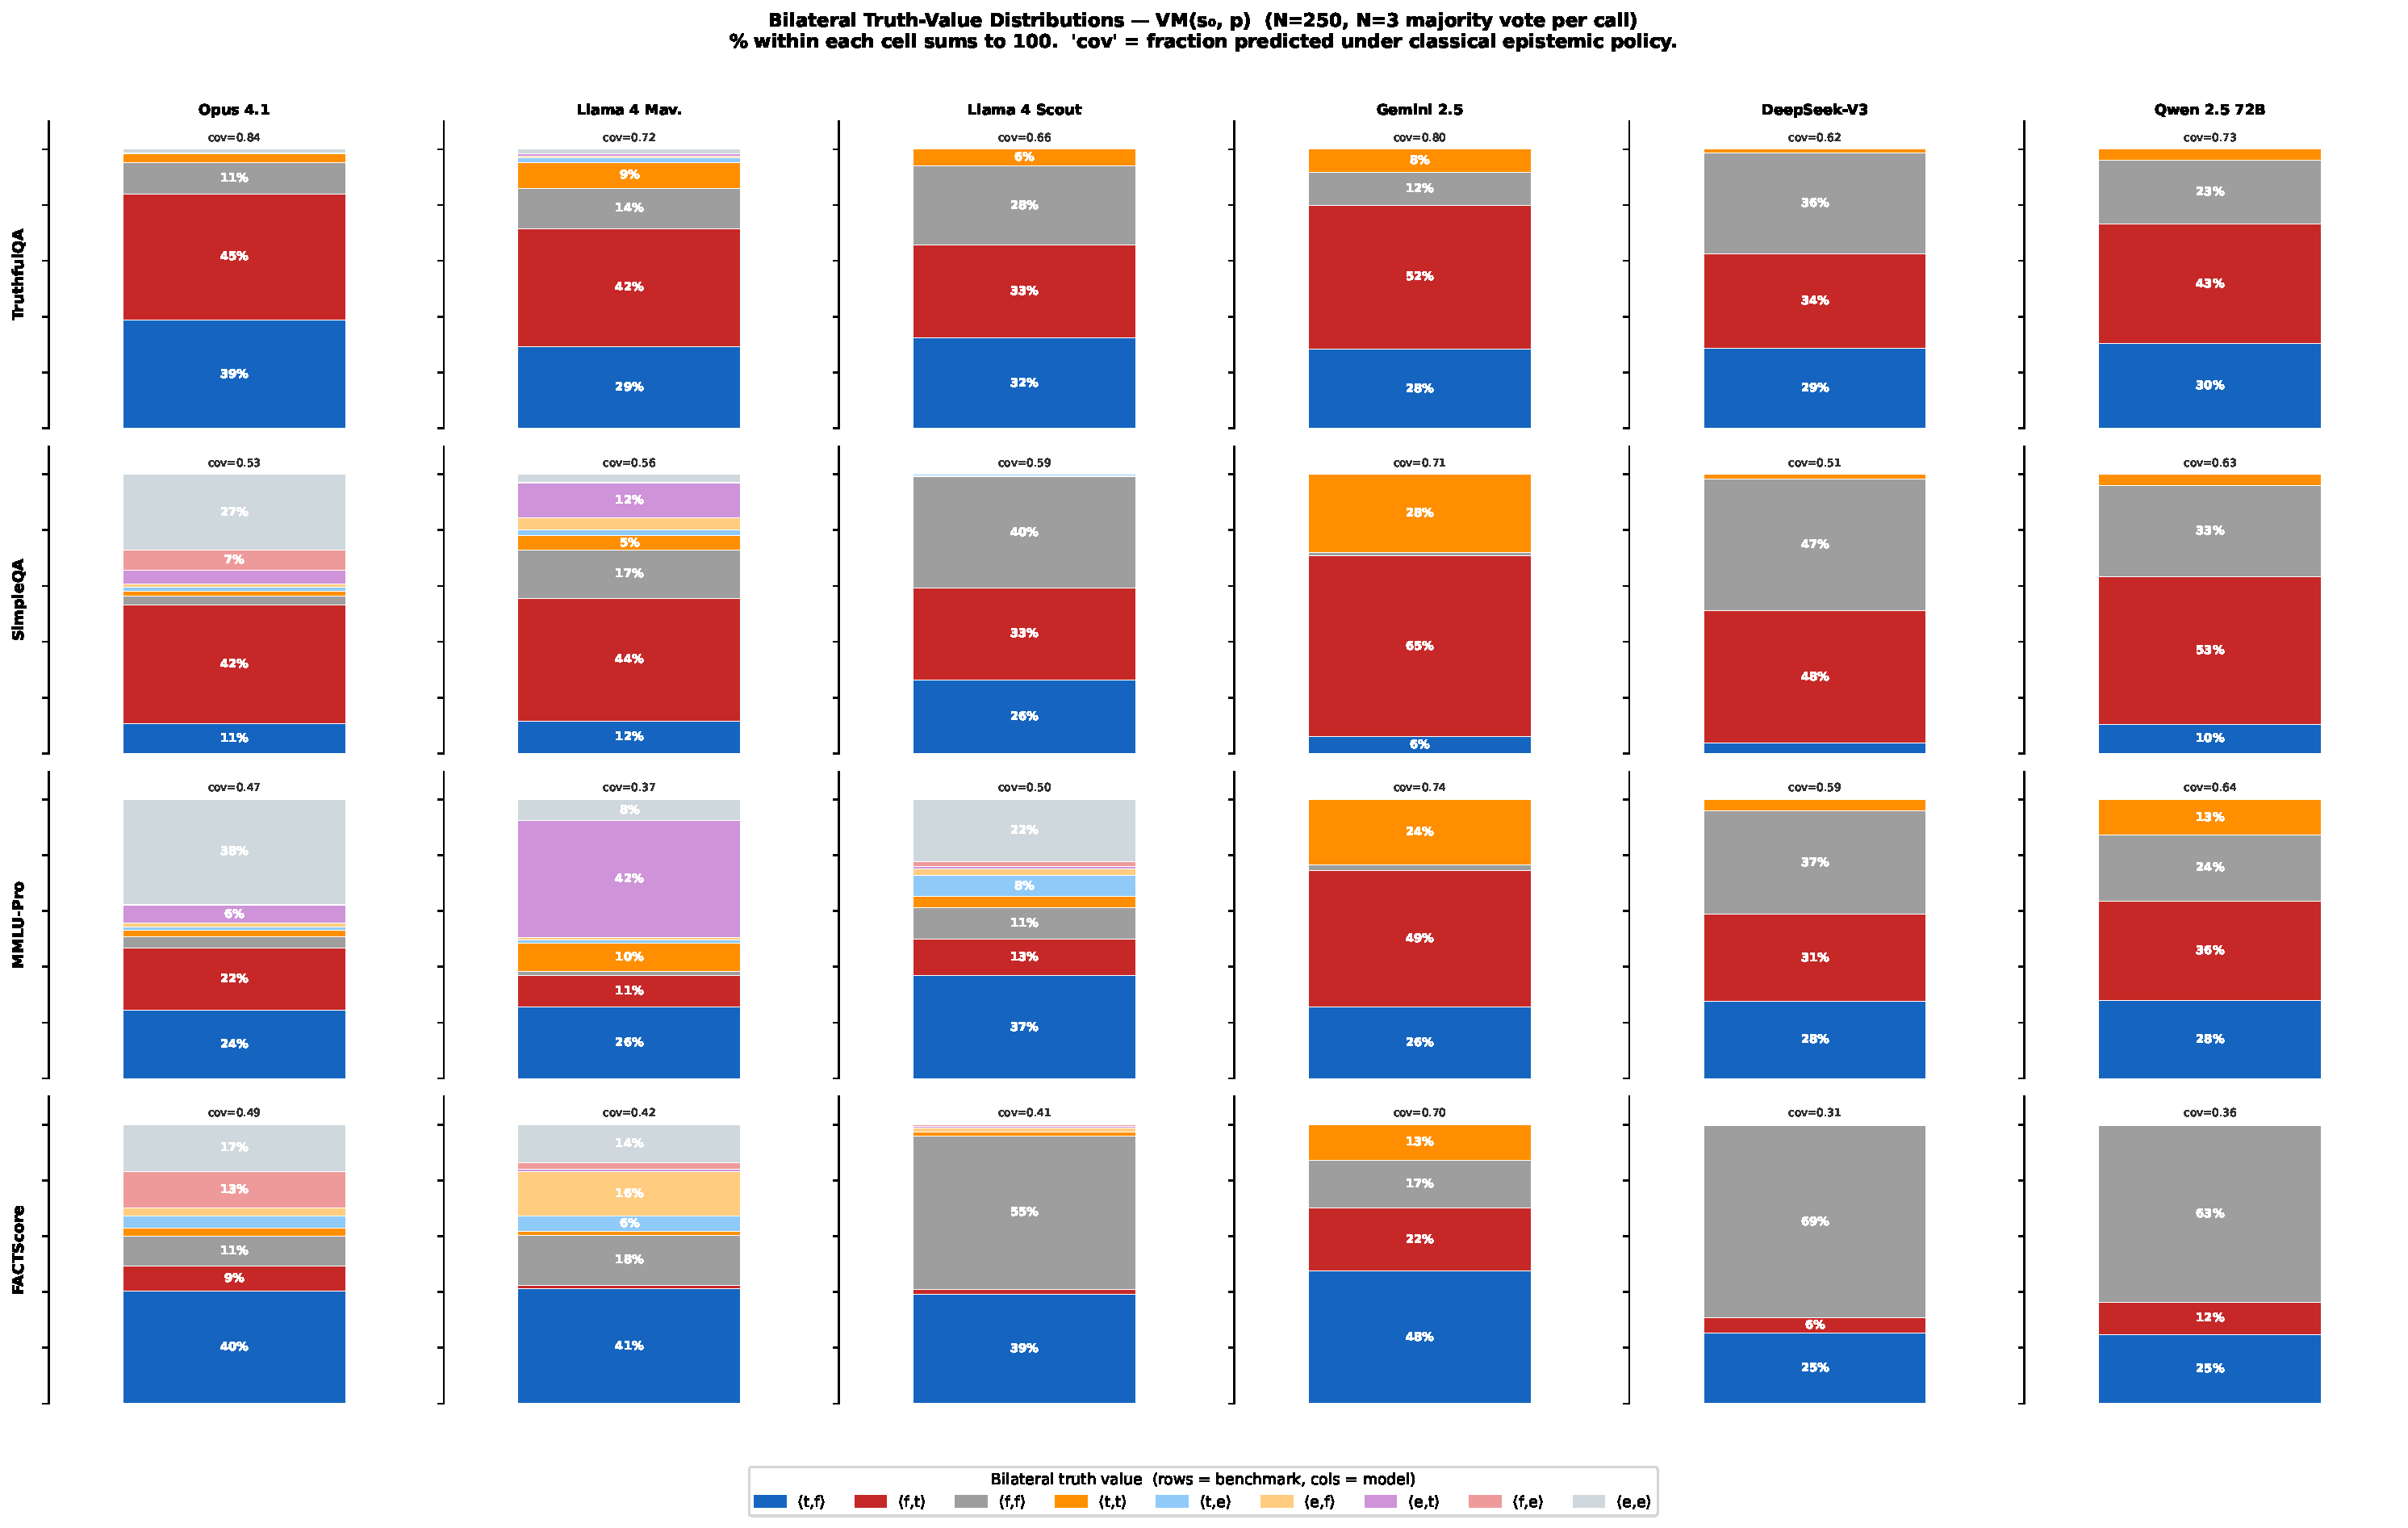
\includegraphics[width=0.97\linewidth, height=0.82\textheight,
                     keepaspectratio]{tv_distributions.pdf}
  \end{center}
\end{frame}

%% ════════════════════════════════════════════════════════════════════════════
%% SLIDE — Diagnostic contrast: ⟨f,f⟩ vs ⟨t,t⟩
%% ════════════════════════════════════════════════════════════════════════════
\begin{frame}{Ignorance $\tv{f}{f}$ and Contradiction $\tv{t}{t}$ Are Not the Same}

  \begin{center}
    
\includegraphics[width=0.97\linewidth, height=0.72\textheight,
                     keepaspectratio]{tv_diagnostic.pdf}
  \end{center}

  \vspace{-2pt}
  \footnotesize
  Both $\tv{f}{f}$ and $\tv{t}{t}$ fall outside $D \cup D^*$ under every epistemic
  policy — both are \emph{``uncertain''} to any unilateral approach.
  \textbf{Bilateral evaluation separates them.}
  $\tv{f}{f}$: near-random ground-truth positive rate (52\%), ternary correctly abstains 65\% of the time.
  $\tv{t}{t}$: ground-truth positive rate skews 68\%, ternary almost never abstains (3\%) —
  it commits on the verification signal while missing the refutation evidence entirely.

\end{frame}

%% ════════════════════════════════════════════════════════════════════════════
%% SLIDE — Modal TV Distributions [[□p]]
%% ════════════════════════════════════════════════════════════════════════════
\begin{frame}{Modal TV Distributions: $[\![\Box p]\!]$}
  \begin{center}
    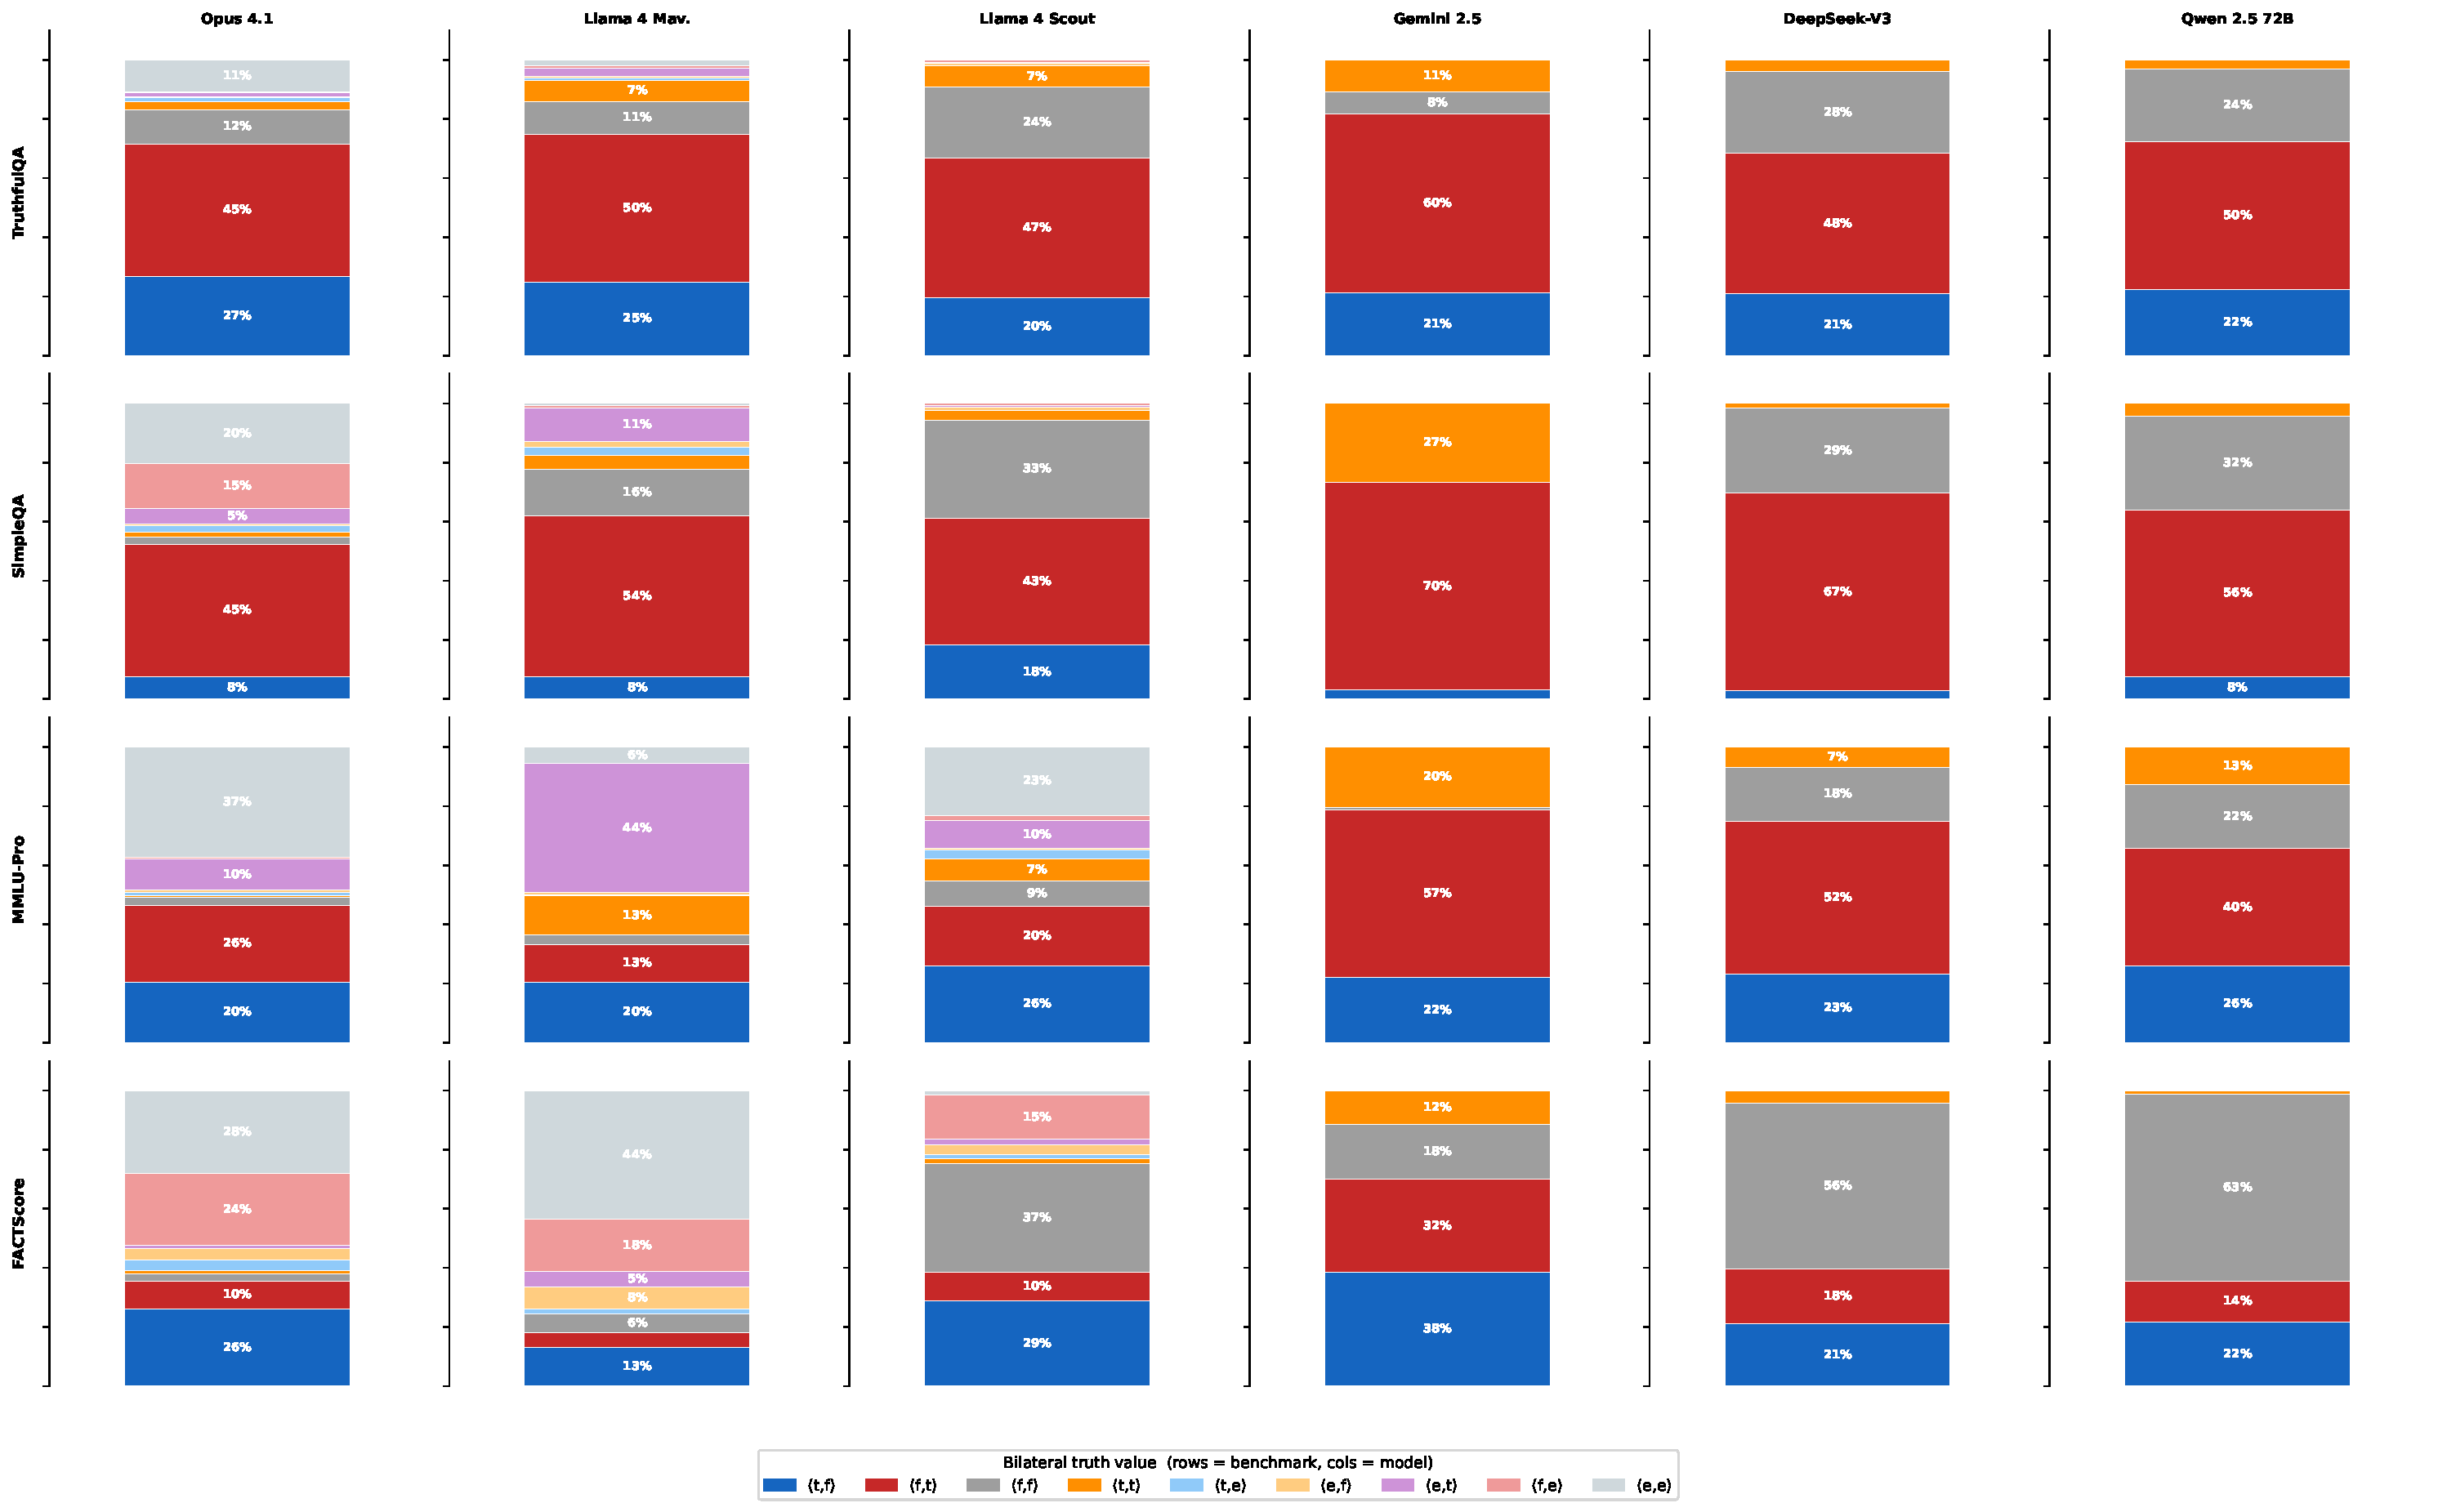
\includegraphics[width=0.97\linewidth, height=0.82\textheight,
                     keepaspectratio]{modal_distributions.pdf}
  \end{center}
\end{frame}

%% ════════════════════════════════════════════════════════════════════════════
%% SLIDE — Source vs Modal Side-by-Side
%% ════════════════════════════════════════════════════════════════════════════
\begin{frame}{$\semp$ vs $[\![\Box p]\!]$: Modal Tightening}
  \begin{center}
    
\includegraphics[width=0.97\linewidth, height=0.82\textheight,
                     keepaspectratio]{src_vs_modal_distributions.pdf}
  \end{center}
\end{frame}

%% ════════════════════════════════════════════════════════════════════════════
%% SLIDE 8 — Empirical Setup
%% ════════════════════════════════════════════════════════════════════════════
\begin{frame}{Empirical Setup}

  \begin{columns}[T]
    \column{0.48\textwidth}
    \textbf{Models} ($\times 6$, open-source-skewed):
    \medskip
    \begin{tabular}{ll}
      \toprule
      Model & Provider \\
      \midrule
      Claude Opus 4.1 & Anthropic \\
      Llama 4 Maverick & Meta \\
      Llama 4 Scout    & Meta \\
      Gemini 2.5 Flash & Google \\
      DeepSeek-V3      & DeepSeek \\
      Qwen 2.5 72B     & Alibaba \\
      \bottomrule
    \end{tabular}

    \column{0.48\textwidth}
    \textbf{Benchmarks} ($\times 4$):
    \medskip
    \begin{tabular}{ll}
      \toprule
      Benchmark & Focus \\
      \midrule
      TruthfulQA & Misconception resistance \\
      SimpleQA   & Factual precision \\
      MMLU-Pro   & Expert knowledge \\
      FACTScore  & Biographical facts \\
      \bottomrule
    \end{tabular}
  \end{columns}

  \medskip

  \small\textbf{Protocol:}
  $N = 250$ assertions per cell (seed = 42, balanced 50/50 +/-);
  $n = 3$ paraphrase variants; bilateral samples = 3 (majority vote).
  Variants generated once per dataset, cached across all models.

  \medskip
  \textbf{Five approaches} compared in a single pass: bilateral (3 policies),
  forced unilateral, ternary, and confidence@0.5.

\end{frame}

%% ════════════════════════════════════════════════════════════════════════════
%% SLIDE — Approach Comparison: avg F1 / Coverage
%% ════════════════════════════════════════════════════════════════════════════
\begin{frame}{Bilateral vs.\ Ternary vs.\ Unilateral: F1 Macro and Coverage}

  \small
  Macro-averages across 6 models per benchmark ($N=250$ each).
  Bilateral uses the paracomplete policy $D=\{\tv{t}{f},\tv{t}{e}\}$.
  \textbf{Bold} = highest F1 in that row.

  \smallskip

  \setlength{\tabcolsep}{5pt}
  \renewcommand{\arraystretch}{1.3}
  \small
  \begin{tabular}{l @{\quad} cc @{\quad} cc @{\quad} cc}
    \toprule
    & \multicolumn{2}{c}{\textbf{Bilateral (PC)}}
    & \multicolumn{2}{c}{\textbf{Ternary}}
    & \multicolumn{2}{c}{\textbf{Unilateral}} \\
    \cmidrule(lr){2-3}\cmidrule(lr){4-5}\cmidrule(lr){6-7}
    \textbf{Benchmark} & F1 & Cov & F1 & Cov & F1 & Cov \\
    \midrule
    TruthfulQA  & .74 & .94 & \textbf{.84} & .84 & .78 & 1.00 \\
    SimpleQA    & .79 & .85 & \textbf{.87} & .72 & .73 & 1.00 \\
    FACTScore   & .45 & .90 & .51          & .62 & \textbf{.60} & 1.00 \\
    \midrule
    \textit{Average} & .66 & .89 & \textbf{.74} & .73 & .70 & 1.00 \\
    \bottomrule
  \end{tabular}

  \medskip\footnotesize
  Ternary achieves the highest F1 on average --- by refusing to answer 27\% of
  assertions.  Unilateral commits on all assertions but cannot express what it
  does not know.  \textbf{Neither can distinguish $\tv{f}{f}$ (ignorance) from
  $\tv{t}{t}$ (contradiction)}: the ternary abstain-rate analysis (previous
  slide) shows why that distinction matters.

\end{frame}

%% ════════════════════════════════════════════════════════════════════════════
%% SLIDE — Modal F1 / Coverage Table
%% ════════════════════════════════════════════════════════════════════════════
\begin{frame}{Coverage and F1 Macro: Source vs.\ Modal}

  \small
  Each cell: \textbf{source\,/\,modal} with delta $(\Delta)$.
  Coverage = fraction of assertions predicted under classical $D=\{\tv{t}{f}\}$.
  F1~macro computed on covered assertions only.

  \medskip

  \setlength{\tabcolsep}{2pt}
  \renewcommand{\arraystretch}{1.15}
  \scriptsize
  \begin{tabular}{l
      S[table-format=1.2] S[table-format=1.2]
      S[table-format=1.2] S[table-format=1.2]
      S[table-format=1.2] S[table-format=1.2]
      S[table-format=1.2] S[table-format=1.2]}
    \toprule
    & \multicolumn{2}{c}{\textbf{TruthfulQA}}
    & \multicolumn{2}{c}{\textbf{SimpleQA}}
    & \multicolumn{2}{c}{\textbf{MMLU-Pro}}
    & \multicolumn{2}{c}{\textbf{FACTScore}} \\
    \cmidrule(lr){2-3}\cmidrule(lr){4-5}\cmidrule(lr){6-7}\cmidrule(lr){8-9}
    \textbf{Model}
      & {Cov} & {F1}
      & {Cov} & {F1}
      & {Cov} & {F1}
      & {Cov} & {F1} \\
    \midrule
    & \multicolumn{8}{l}{\tiny src\,/\,modal\quad(\(\Delta\) modal\(-\)src)} \\[-2pt]
    Opus 4.1
      & {.74/.72\;(-.02)} & {.91/.86\;(-.05)}
      & {.52/.52\;(.00)}  & {.93/.87\;(-.06)}
      & {.43/.46\;(+.04)} & {.90/.84\;(-.06)}
      & {\textcolor{falsered}{.49/.36\;(-.14)}}
        & {\textcolor{trueblue}{.52/.59\;(+.07)}} \\
    Llama 4 Mav.
      & {.70/.75\;(+.04)} & {.77/.74\;(-.03)}
      & {.57/.62\;(+.05)} & {.86/.73\;(-.13)}
      & {.36/.33\;(-.02)} & {.79/.80\;(+.01)}
      & {\textcolor{falsered}{.42/.18\;(-.24)}}
        & {\textcolor{trueblue}{.43/.50\;(+.07)}} \\
    Llama 4 Scout
      & {.62/.67\;(+.04)} & {.72/.63\;(-.10)}
      & {.63/.61\;(-.02)} & {.91/.88\;(-.03)}
      & {.48/.46\;(-.02)} & {.74/.77\;(+.03)}
      & {.42/.38\;(-.04)}
        & {\textcolor{trueblue}{.40/.56\;(+.16)}} \\
    Gemini 2.5~F.
      & {.81/.82\;(+.01)} & {.83/.76\;(-.06)}
      & {.71/.73\;(+.02)} & {.62/.52\;(-.10)}
      & {.74/.79\;(+.05)} & {.78/.75\;(-.03)}
      & {.69/.70\;(+.01)} & {.64/.68\;(+.04)} \\
    DeepSeek-V3
      & {.66/.68\;(+.02)} & {.81/.75\;(-.06)}
      & {.60/.70\;(+.10)} & {.72/.52\;(-.20)}
      & {.66/.75\;(+.09)} & {.78/.76\;(-.02)}
      & {.38/.40\;(+.02)} & {.57/.58\;(+.01)} \\
    Qwen 2.5~72B
      & {.73/.72\;(-.01)} & {.83/.78\;(-.05)}
      & {.63/.64\;(+.01)} & {.77/.73\;(-.05)}
      & {.64/.66\;(+.02)} & {.76/.75\;(-.01)}
      & {.36/.36\;(-.01)} & {.57/.55\;(-.01)} \\
    \bottomrule
  \end{tabular}

  \smallskip\footnotesize
  \textcolor{falsered}{Red}: large PSK-driven coverage loss (Llama\,4 Mav.\ $-$0.24 on FACTScore).\\
  \textcolor{trueblue}{Blue}: F1 \emph{rises} under modal filtering —
  prompt-sensitive lucky predictions are correctly withheld.

\end{frame}

%% ════════════════════════════════════════════════════════════════════════════
%% SLIDE 9 — Empirical Results: Bilateral Distributions
%% ════════════════════════════════════════════════════════════════════════════
\begin{frame}{Empirical Results: Bilateral Distributions}

  \begin{columns}[T]
    \column{0.55\textwidth}
    \textbf{Key findings across 24 model $\times$ benchmark cells:}
    \begin{itemize}\setlength\itemsep{5pt}
      \item \textcolor{trueblue}{$\tv{t}{f}$ (\textsc{True})} dominates \textbf{TruthfulQA} —
            models are mostly confident and uncontested on factual questions
      \item \textcolor{ignorgray}{$\tv{f}{f}$ (\textsc{Ignorance})} dominates \textbf{FACTScore}
            — models systematically cannot verify \emph{or} refute biographical facts
      \item \textbf{MMLU-Pro} shows lowest classical coverage — questions require
            genuine uncertainty; paraconsistent policy recovers significant F1
      \item \textcolor{ignorgray}{$\tv{f}{f}$} and \textcolor{contramber}{$\tv{t}{t}$}
            are both ``uncertain'' under unilateral evaluation but are observably
            \emph{different} states with different diagnostic implications
    \end{itemize}

    \column{0.42\textwidth}
    \begin{block}{The diagnostic reading}
      High $\tv{f}{f}$ on FACTScore is not a failure of bilateral evaluation
      — it is the framework \textbf{correctly diagnosing} that the model has
      no relevant training signal for biographical claims.

      \medskip
      Unilateral evaluation would report the same result as MMLU-Pro: low accuracy.
      Bilateral evaluation distinguishes \emph{why}.
    \end{block}
  \end{columns}

  \medskip\pause
  \small
  \textbf{Bilateral $\approx$ ternary on covered examples.}
  The contribution is not accuracy improvement — it is the richer
  epistemic characterisation of the non-covered cases.

\end{frame}

%% ════════════════════════════════════════════════════════════════════════════
%% SLIDE 10 — Frame Conditions: Empirical Support
%% ════════════════════════════════════════════════════════════════════════════
\begin{frame}{Frame Conditions: Empirical Support for System B}

  \begin{columns}[T]
    \column{0.5\textwidth}
    \begin{block}{T axiom: $[\![\Box p]\!] \leq_t \semp$ \hfill \textcolor{green!60!black}{Confirmed}}
      \small
      Necessity can only \emph{weaken} the source verdict.
      If $[\![p]\!] = \langle t,f\rangle$ then $[\![\Box p]\!] \in
      \{\langle t,f\rangle, \langle t,e\rangle, \langle e,f\rangle, \ldots\}$
      — never strictly more designated.\\[4pt]
      Tested on 277 cases where removing $s_0$ from the
      aggregation would change the result:
      \textbf{0 violations} across all 6 models $\times$ 4 benchmarks.
    \end{block}

    \column{0.46\textwidth}
    \begin{block}{B axiom: $\semp \in D \Rightarrow [\![\Box p]\!]_{s_i} \in D$ \hfill \textcolor{orange!80!black}{Consistent}}
      \small
      If $p$ holds at $s_0$, it should hold modally from any variant too.
      Proxy test: recompute $[\![\Box p]\!]$ treating each $s_i$ as the new
      source in place of $s_0$. Does the designation result agree?\\[4pt]
      \textbf{95.7\%} agreement (6{,}300 model$\times$question pairs,
      each tested 3--4$\times$ across variants).\\[4pt]
      Theoretical grounding: paraphrase accessibility is symmetric
      by construction.
    \end{block}
  \end{columns}

  \medskip\pause

  \begin{block}{Completeness: the Kamide--Shramko translation}
    \small $\BBL$ is sound and complete w.r.t.\ system~B frames via translation
    $\tau$ to classical modal logic.
    \textbf{Def.~19} ($\tau_D(\varphi) = \varphi_v \wedge \varphi^1_r$) is the
    \emph{only} policy-sensitive part — the rest is frame-condition agnostic.
    Metatheoretic results (decidability, complexity)
    are inherited from classical modal T/B.
  \end{block}

\end{frame}

%% ════════════════════════════════════════════════════════════════════════════
%% SLIDE 11 — Formal Reasoning: Defeasible Derivability Oracles
%% ════════════════════════════════════════════════════════════════════════════
\begin{frame}{Formal Reasoning with Defeasible Derivability Oracles}

  \begin{block}{Modal modus ponens}
    \[
      [\![\Box p]\!] \in D \;\wedge\; [\![\Box(p \to q)]\!] \in D
      \;\;\Longrightarrow\;\;
      [\![\Box q]\!] \in D
    \]
    The LLM evaluates $[\![\Box p]\!]$ and $[\![\Box(p{\to}q)]\!]$ independently.
    The logic derives $[\![\Box q]\!]$.
    \textbf{The model never performs the inference} — only the oracle queries.
  \end{block}

  \medskip

  \small
  \begin{columns}[T]
    \column{0.48\textwidth}
    \textbf{In compound AI systems:}
    \begin{itemize}\setlength\itemsep{3pt}
      \item \textbf{Multi-hop reasoning}: bilateral values propagate through
            inference chains; errors are formally tracked, not silently absorbed
      \item \textbf{RAG pipelines}: $\tv{t}{t}$ surfaces conflicting
            retrieved vs.\ prior evidence rather than masking it
      \item \textbf{Multi-model aggregation}: conjunction/disjunction of
            bilateral values is formal, not a voting heuristic
    \end{itemize}

    \column{0.48\textwidth}
    \textbf{Why current pipelines lack this:}
    \begin{itemize}\setlength\itemsep{3pt}
      \item Chain-of-thought asks the LLM to \emph{perform} the inference
            — unaccountable and unverifiable
      \item Confidence scores conflate ignorance $\tv{f}{f}$
            and contradiction $\tv{t}{t}$
      \item No formal criterion for when to trust a composed result
    \end{itemize}
  \end{columns}

  \medskip\pause
  \small
  $\BBL$ provides the \textbf{formal infrastructure} that makes LLM outputs usable
  as inputs to rigorous inference.
  Not: make LLMs reason logically. Rather: \textbf{reason logically using LLMs}.

\end{frame}

%% ════════════════════════════════════════════════════════════════════════════
%% SLIDE 12 — Open Questions
%% ════════════════════════════════════════════════════════════════════════════
\begin{frame}{Open Questions}

  \small
  \begin{enumerate}\setlength\itemsep{5pt}

    \item \textbf{Neighbourhood semantics} —
          non-normal modal operators for LLMs that do not respect the
          distribution axiom~K; more principled basis for the accessibility structure

    \item \textbf{Systematic $D$-parameterisation study} —
          how does $(D, D^*)$ affect coverage, F1, and calibration?
          LP-$\BBL$ and K3-$\BBL$ as proof-theoretic targets

    \item \textbf{Multi-agent $\BBL$} —
          different LLMs instantiating different accessibility relations
          $R_{\mathcal{M}_1}, R_{\mathcal{M}_2}$; formal aggregation across models

    \item \textbf{Dynamic operators} —
          belief revision as modal transition; fine-tuning as a map
          $\mathcal{M} \to \mathcal{M}'$ with formally characterised effects on $V_\mathcal{M}$

    \item \textbf{Definitive symmetry test} —
          generate variants-of-variants to empirically confirm the B~axiom,
          or establish system~T + theoretical symmetry as the right frame class

  \end{enumerate}

\end{frame}

%% ════════════════════════════════════════════════════════════════════════════
%% SLIDE 13 — Conclusion
%% ════════════════════════════════════════════════════════════════════════════
\begin{frame}{Conclusion}

  \begin{block}{The thesis}
    \textit{Don't try to get LLMs to reason logically.
    Build a logic that reasons using LLMs as defeasible derivability oracles.}
  \end{block}

  \medskip

  \small\textbf{$\BBL$ delivers:}
  \begin{itemize}\setlength\itemsep{3pt}
    \item A \textbf{sound and complete} bilateral modal logic grounded in LLM evaluation
    \item A \textbf{parameterised family} $\BBL_{D,D^*}$ of epistemic policies
          with a unified proof-theoretic treatment
    \item A \textbf{modal operationalisation} of knowledge stability via $[\![\Box p]\!]$,
          diagnosing prompt-sensitive knowledge before it enters inference chains
    \item \textbf{Empirically confirmed} frame conditions: T axiom (277/277),
          B axiom consistent (95.7\% permuted agreement)
    \item A \textbf{formal basis} for reasoning about composed LLM outputs in
          compound AI systems
  \end{itemize}

  \medskip

  \begin{center}
    \small
    \texttt{arxiv.org/abs/2507.09751} \quad$\cdot$\quad
    Code \& data: \texttt{github.com/bradleynallen/bilateral-truth}
  \end{center}

\end{frame}

\end{document}

